\documentclass[10pt,DIV=23,landscape]{scrartcl}
\usepackage{dominatrix}

\pagenumbering{gobble}

\usepackage{paracol}
\setlength{\columnsep}{4em}
%\setlength{\columnseprule}{0.4pt}

\usepackage{solarized-light}
\lstset{
language=R
}
\title{Java Style Guide}
\subject{CS 3134 Data Structures and Algorithms}
\author{Linan Qiu\\\texttt{lq2137}}
\begin{document}
\maketitle

\begin{abstract}
This is a short but important collection of coding standards that we
expect you to follow for this class. You will find that adhering to this
code results in readable, maintainable, and easy to debug code. Beyond
this class, you will find that good code style is essential not only for
yourself but also for any large codebase engineered by a team of
developers.

We do not claim ownership over these tips. Rather, they are inspired by
\href{https://google.github.io/styleguide/javaguide.html}{Google's Java
Style Guide} which we encourage you to spend 7 minutes reading. Multiple
TAs over the generations (Linan Qiu, James Lin, Andrew Goldin, Madhavan
Somanathan) have also contributed to this guide.
\end{abstract}

\section{Source File Basics}\label{source-file-basics}

\begin{paracol}{2}
\begin{leftcolumn}
\subsection{File Name}\label{file-name}

Source file name consists of the name of the class plus the
\lstinline{.java} extension.
\end{leftcolumn}

\begin{rightcolumn}
\subsection{File Encoding}\label{file-encoding}

Source files can be either UTF-8 or ASCII.
\end{rightcolumn}
\end{paracol}

\subsection{File Header}\label{file-header}

\begin{paracol}{2}
\begin{leftcolumn}
Include your name, UNI, and description of the file in each Java source
file that you write. This allows you to quickly identify the author of
the code and the code's purpose.
\end{leftcolumn}

\begin{rightcolumn}
\begin{lstlisting}
/* James Lin
 * jl3782
 * HanSolo.java - killed
 */

public class HanSolo {
  // ...
}
\end{lstlisting}
\end{rightcolumn}
\end{paracol}

\subsection{Use Default Package}\label{use-default-package}

\begin{paracol}{3}
\begin{nthcolumn}{0}
\textbf{Use the default package for all your classes}. Since this course does not require packages, you usually end up creating
classes within packages as a result of IDEs' over-helpfulness. Make sure
you leave the package row empty when you create a new class in your IDE
(screenshot attached for Eclipse) even though it warns you otherwise.
While it may be a good idea to put your classes in packages for large
codebases, you won't need them for this class and you will instead give
your TA compilation troubles. \textbf{Do not create your class within a
package.}
\end{nthcolumn}

\begin{nthcolumn}{1}
That means instead of declaring your class file as such:
\begin{lstlisting}
package somepackage;

public class Bulbasaur {
  // ...
}
\end{lstlisting}

You should only have

\begin{lstlisting}
public class Bulbasaur {
  // ...
}
\end{lstlisting}
\end{nthcolumn}

\begin{nthcolumn}{2}
\begin{figure}[H]
\centering
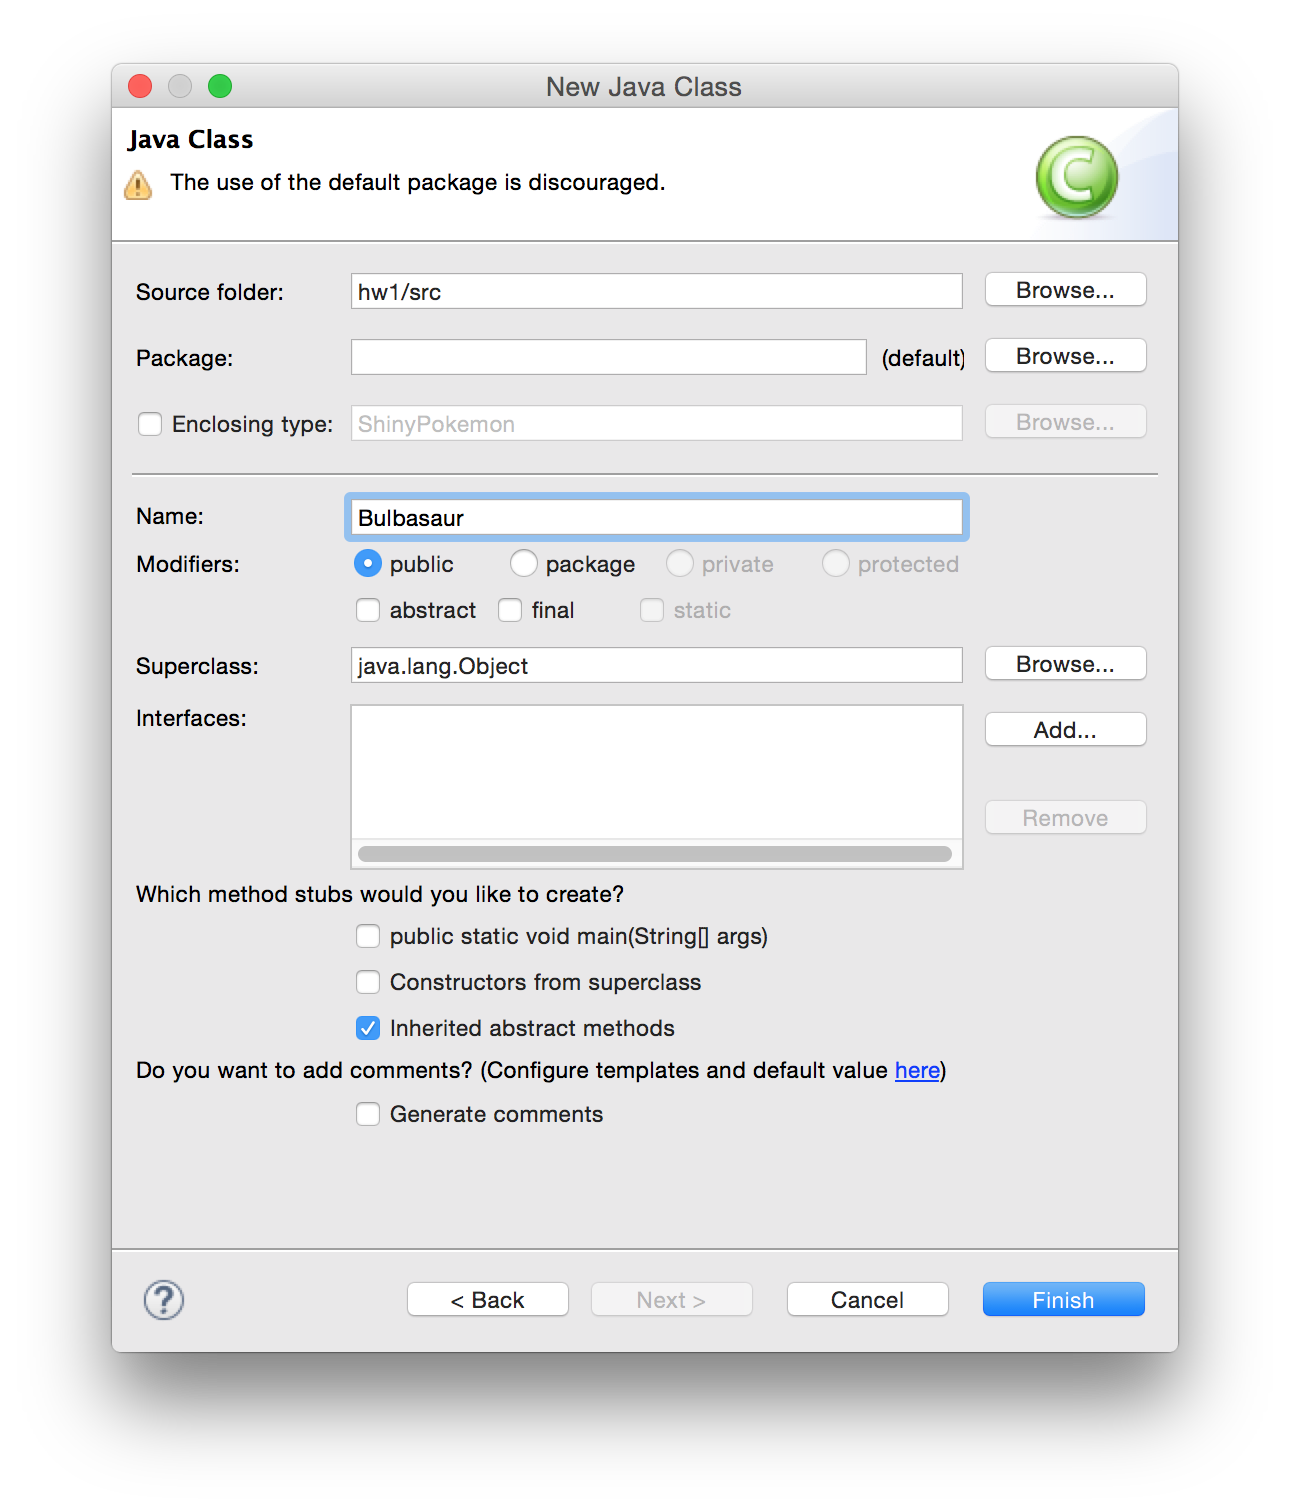
\includegraphics[width=0.25\textwidth]{default-package.png}
\caption{Creating a new class in Eclipse under the default package}
\end{figure}
\end{nthcolumn}

\end{paracol}

\section{Formatting}\label{formatting}

\subsection{Brace Styles}\label{brace-styles}

\begin{paracol}{2}
\begin{leftcolumn}
You are required to choose between the K\&R style or Allman style for
creating blocks of code (e.g.~in \lstinline{if} blocks, \lstinline{while} and
\lstinline{for} loops, defining classes etc). \textbf{Be consistent}
throughout your code (ie. don't switch between styles in your code).
\end{leftcolumn}

\begin{rightcolumn}
\begin{lstlisting}
// K&R
for(int i = 0; i < array.length; i++) {
  System.out.println(array[i]);
}

// Horstmann
for(int i = 0; i < array.length; i++)
{
  System.out.println(array[i]);
}
\end{lstlisting}
\end{rightcolumn}
\end{paracol}

\subsection{Use Braces Wherever
Optional}\label{use-braces-wherever-optional}

\begin{paracol}{2}
\begin{leftcolumn}
Braces are used with \lstinline{if}, \lstinline{else}, \lstinline{for},
\lstinline{do} and \lstinline{while} statements, even when the body is empty
or contains only a single statement.
\end{leftcolumn}

\begin{rightcolumn}
\begin{lstlisting}
// while this compiles
for (int i = 0; i < array.length; i++)
  System.out.println(array[i]);

// you should instead do this
for(int i = 0; i < array.length; i++) {
  System.out.println(array[i]);
}
\end{lstlisting}
\end{rightcolumn}
\end{paracol}

\subsection{Indentation}\label{indentation}

\begin{paracol}{2}
\begin{leftcolumn}
You can indent using \textbf{tabs, 2 spaces, or 4 spaces}. We allow tabs
for convenience. However, in the industry, most companies (including
Google) requires that tabs be translated into spaces. Most IDEs / text
editors do this automatically should you set it up to do so.
\end{leftcolumn}

\begin{rightcolumn}
\begin{lstlisting}
// indentation using 2 spaces
int i = 0;
while (i < array.length) {
  double random = Math.random();
  if (random < 0.5) {
    array[i] = 0;
  } else {
    array[i] = i;
  }
}
\end{lstlisting}
\end{rightcolumn}
\end{paracol}

\subsection{Line Length}\label{line-length}

\begin{paracol}{2}
\begin{leftcolumn}
Keep your lines at \textbf{80 characters or under}. You will need to
break up or wrap lines and comments that are longer than this. Again,
most IDEs can do this for you.
\end{leftcolumn}

\begin{rightcolumn}
\begin{lstlisting}
String str = "This is a long strong " +
    "that needs to be broken up";
\end{lstlisting}
\end{rightcolumn}
\end{paracol}

\subsection{White Space}\label{white-space}

\begin{paracol}{2}
\begin{leftcolumn}
Place a blank line between each new thought. This allows your reader to
follow your thought process step-by-step and keeps your code from
getting cluttered. The code below demonstrates a program getting an
object's data then displaying the information. The break shows the
separation in thought even though the code is in a single method.
\end{leftcolumn}

\begin{rightcolumn}
\begin{lstlisting}
public boolean canDrive(Person person) {
  int age = person.getAge();

  return age >= 16;
}
\end{lstlisting}
\end{rightcolumn}
\end{paracol}

\section{Naming}\label{naming}

\begin{paracol}{3}
\begin{nthcolumn}{0}
\subsection{Class Names}\label{class-names}

Class names are written in
\href{https://google.github.io/styleguide/javaguide.html\#s5.3-camel-case}{UpperCamelCase}
(e.g. \lstinline{HanSolo} or \lstinline{BinaryTree}) Class names are typically
nouns or noun phrases. (e.g. \lstinline{Character} or
\\ \lstinline{ImmutableList}). Interface names may also be nouns or noun
phrases (e.g. \lstinline{List}), but may sometimes be adjectives or
adjective phrases instead (for example, \lstinline{Readable}).

\end{nthcolumn}
\begin{nthcolumn}{1}

\subsection{Variable Names}\label{variable-names}

Variable names (static or otherwise) are written in
\href{https://google.github.io/styleguide/javaguide.html\#s5.3-camel-case}{lowerCamelCase}.

These names are typically nouns or noun phrases. For example,
\lstinline{computedValues} or \lstinline{index}.

\end{nthcolumn}
\begin{nthcolumn}{2}
\subsection{Method Names}\label{method-names}

Method names are written in \href{https://google.github.io/styleguide/javaguide.html\#s5.3-camel-case}{lowerCamelCase}
(e.g. \lstinline{kissLeia} or \lstinline{toString}).

Method names are typically verbs or verb phrases. For example,
\lstinline{sendMessage} or \lstinline{stop}.
\end{nthcolumn}
\end{paracol}

\subsection{Constant Names}\label{constant-names}

\begin{paracol}{2}
\begin{leftcolumn}
Constant names use \lstinline{CONSTANT_CASE}: all uppercase letters, with
words separated by underscores.
\end{leftcolumn}

\begin{rightcolumn}
\begin{lstlisting}
public static final int ANSWER_TO_UNIVERSE = 42;
public static final String WARNING = "Shall not pass";
\end{lstlisting}
\end{rightcolumn}
\end{paracol}

\subsection{Meaningful Names}\label{meaningful-names}

Give your classes, variables, and methods meaningful names. For example,
instead of calling a class \lstinline{Robot} (not informative, since all
programs are robots), call it \lstinline{Calculator}. Instead of calling a
variable \lstinline{number}, call it \lstinline{height} if it is used to
denote the height of a person.

\subsection{Avoid Hardcoding Magic
Numbers}\label{avoid-hardcoding-magic-numbers}

\begin{paracol}{2}
\begin{leftcolumn}
Avoid hardcoding any constants that bear significance affecting the
output of your program. If you have to hardcode them, give them
meaningful names.
\end{leftcolumn}

\begin{rightcolumn}
\begin{lstlisting}
// Bad
public double weight(double mass) {
  return mass * 9.81;
}

// Good
public static final double GRAVITY = 9.81;

public double weight(double mass) {
  return mass * GRAVITY;
}
\end{lstlisting}
\end{rightcolumn}
\end{paracol}






\end{document}
